\documentclass{article}
\usepackage[utf8]{inputenc}
\usepackage[russian]{babel}
\usepackage{graphicx}
\usepackage{amsmath}
\usepackage{breqn}
\usepackage{wrapfig}
\usepackage{float}
\usepackage{multirow}
\usepackage{caption}
\usepackage{subcaption}

\graphicspath{ {./data/images} }
\author{Александр Романов Б01-107}
\date{}
\title{4.7.3 Поляризация}

\begin{document}
\maketitle
\section{Введение}

\subsection{Цель работы}
Ознакомление с методами получения и анализа поляризованного света.
\subsection{В работе используются}
Оптическая скамья с осветителем; зелёный светофильтр; два поляроида; чёрное зеркало; полированная эбонитовая
пластинка; стопа стеклянных пластинок; слюдяные пластинки разной толщины; пластинки в 1/4 и 1/2 длины волны;
пластинка в одну длину волны для зелёного света (пластинка чувствительного оттенка).
\subsection{Теоретическая справка}
Сдвиг фаз поляризованной волны при прохождении через двоякопреломляющую пластинку:

\begin{figure}[H]
    \centering
    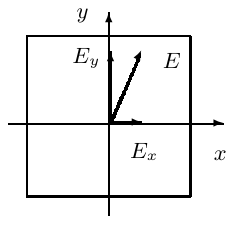
\includegraphics[width=0.5\textwidth]{polarized-decomposition.png}
    \caption{Разложение линейно поляризованного света по главным направлениям
    двоякопреломляющей пластинки}
\end{figure} 

\[ \Delta\varphi = \frac{2\pi}{m} = kd\left(n_x - n_y\right) \]
где \(k\) - волновое число (в пустоте), d - толщина кристаллической пластинки.

При сложении двух взаимно перпендикулярных колебаний обладающих некоторым сдвигом фаз, образуется
колебание, поляризованное по элипсу. Есть разные случаи:

\begin{figure}[H]
    \centering
    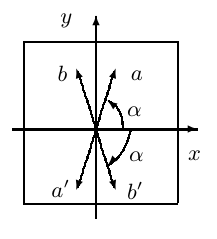
\includegraphics[width=0.5\textwidth]{oscillation-rotate.png}
    \caption{Поворот направления колебаний с помощью пластинки в \(\lambda/2\)}
\end{figure} 

\begin{enumerate}
    \item Пластинка даёт сдвиг фаз в \(2\pi\) (Пластинка в длину волны \(\lambda\))
Результат: поляризованная волна с тем же направлением колебаний.
    \item Пластинка даёт сдвиг фаз в \(\pi\) (Пластинка в \(\lambda/2\))
Результат: Направление колебаний поляризованной волны повёрнуто относительно начального.
    \item Пластика даёт сдвиг фаз в \(\pi/2\) (Пластинка в \(\lambda/4\))
Результат: Элипс, главные оси которого совпадают с \(x\) и \(y\).
\end{enumerate}

\section{Работа}

\subsection{Определение разрешённых направлений поляроида}
Разместим на оптической скамье осветитель \(S\), поляроид \(P_1\) и чёрное зеркало.

\begin{figure}[H]
    \centering
    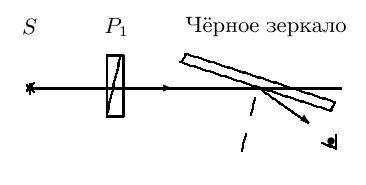
\includegraphics[width=0.7\textwidth]{polaroid-direction.png}
    \caption{Определение разрешённого направления поляроида}
    \label{fig:pol-dir}
\end{figure} 

Поворачивая поляроид вокруг направления луча, а чёрное зеркало вокруг вертикальной оси, методом последовательных приближений,
добьёмся наименьшей яркости отражённого пятна. Определим разрешённое направление поляроида: для \(P_1\) разрешённое
направление соответствует отметке 352 на его ободе. Заменим чёрное зеркало вторым поляроидом и определим его
разрешённое направление: отметка 300 на его ободе.

\subsection{Определение показателя преломления эбонита}

На схеме с Рис. \ref{fig:pol-dir} заменим чёрное зеркало эбонитовой пластиной. Поворачивая пластину, по лимбу определим
угол брюстера: 
\[ \varphi_b = 55^\circ \]
Неточность оценим \(\pm 5^\circ\)

Добавим в схему светофильтр \(\Phi\) и повторим измерения. Получим значение Угла Брюстера:
\[ \varphi_b = 52^\circ \]

По полученному значению угла Брюстера расчитаем показатель преомления эбонита:
\[ n = \tan{\varphi_b} = \tan{55^\circ} = 1.42 \]

Что отличается от табличного \(\left( n = 1.6 - 1.7 \right)\). Что может быть обусловлено наличием окислений
на эбонитовом образце (Их было видно невооружённым глазом).

\subsection{Исследование характера поляризации света в преломлённом и отражённом от стопы лучах}

Поставим вместо эбонитового зеркаа стопу стеклянных пластинок под углом Брюстера.

\begin{figure}[H]
    \centering
    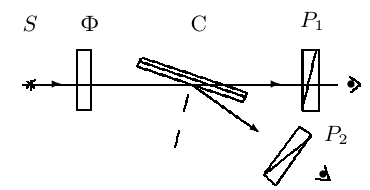
\includegraphics[width=0.7\textwidth]{stack.png}
    \caption{Исследование стопы}
    \label{fig:stack}
\end{figure} 

Осветим стопу поляризованным светом и, рассматривая через поляроиды (Рис. \ref{fig:stack}) отражённный от стопы и преломлённый лучи, определим в них ориентацию вектора E:
\[ E_{refr} = 91^\circ \text{от горизонтали}\]
\[ E_{refl} = 82^\circ \text{от вертикали} \]

\subsection{Определение главных направлений двоякопреломляющих пластин}

\begin{figure}[H]
    \centering
    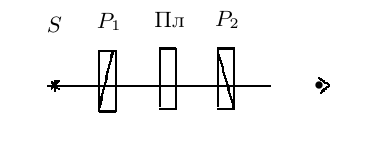
\includegraphics[width=0.7\textwidth]{main-directions.png}
    \caption{Определение главных направлений в пластинах}
    \label{fig:main-dir}
\end{figure} 

Поставим кристаллическую пластинку между скрещенными поляроидами (Рис. \ref{fig:main-dir}).

Вращая пластину вокруг направления луча и наблюдая за интенсивностью света, проходящего через второй поляроид,
определим, при каком условии главные направления пластинки совпадают с разрешёнными направлениями поляроидов:

-- Совпадает с \(P_1\): \(174^\circ\)

-- Совпадает с \(P_2\): \(221^\circ\)

Повторим для второй пластинки:

-- Совпадает с \(P_1\): \(291^\circ\)

-- Совпадает с \(P_2\): \(336^\circ\)


\subsection{Определим какая из пластинок \(\lambda/2\), а какая \(\lambda/4\)}

Добавим к схеме на Рис. \ref{fig:main-dir} зелёный фильтр.

Установим разрешённое направление \(P_1\) горизонтально, а главные направления исследуемой пластинки под углом 
в \(45^\circ\) к горизонтали.

С помощью второго поляроида установим, какую поляризацию имеет свет, прошедший пластинку: круговую или линейную 
с переходом в другой квадрант.

Было выяснено что Первая пластинка это \(\lambda/4\), а вторая - \(\lambda/2\)

\subsection{Определим "Быструю" и "Медленную" оси в пластинке \( \lambda/4 \)}

\begin{figure}[H]
    \centering
    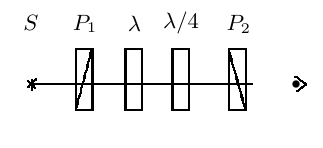
\includegraphics[width=0.7\textwidth]{high-low-speed-direction.png}
    \caption{Определение направлений большей и меньшей скорости}
    \label{fig:high-low}
\end{figure} 

Поставим между скрещенными поляроидами пластинку чувствительного оттенка, имеющую вид стрелки, и убедимся, что эта 
пластинка не меняет поляризацию зелёного света.

Уберём зелёный фильтр и убедимся что стрелка имеет пурпурный цвет. Это происходит из-за того, что зелёный свет задержи
вается вторым поляроидом, а синяя и красная компоненты проходят.

Добаивм к схеме пластину \( \lambda/4 \) (Рис. \ref{fig:high-low}), главные направления которой совпадают с главными направлениями
пластины \(\lambda\) и ориентированы под углом \(45^\circ\) к разрешённым направления скрещенных поляроидов.

При повороте рейтера на \( 180^\circ \) вокруг вертикальной оси цвет стрелки меняется от зелёно-голубого до оранжего-жёлтого.
В случае оранжего-жёлтого "быстрые" оси обоих пластин совпадают, т.к. стрелка немного красненькая и с \( \lambda/4 \) это усиливается,
а если повернуть стрелку, то наоборот ослабляется. В одном положении проникают волны большой частоты, а во второ - мвленькой.

\subsection{Интерференция поляризованных лучей}

Расположим между скрещенными поляроидами мозаичную слюдяную пластинку. Она собрана из 4 узких полосок слюды, лежащих по сторонам квадрата.
(две полоски \( \lambda/4 \) и по одной \( \lambda/2 \) и \( 3\lambda/4 \)). В центральном квадратике слюды нет. Главные
направления всех пластинок ориентированы вдоль сторон квадрата.

Вращая пластинку будем наблюдать за изменениями в отдельном квардратике. Он темнеет и светлеет.

Теперь не трогая пластинки, будем вращать второй поляроид. Теперь все квадратики кроме центрального не тускнеют, а приобретают
и теряют яркие цвета.

\section{Выводы}

В ходе выполнения работы:
\begin{enumerate}
    \item Были изучены методы получения поляризованного света, явление угла Брюстера.
    \item Были определены разрешённые направления поляроидов \(P_1\) и \(P_2\): \(352^\circ\) и \(300^\circ\) соответственно.
    \item Был оценён показатель преломления у эбонита (\(n = 1.42\)). Это значение отличается от табличного \(\left( n = 1.6 - 1.7 \right)\). 
Что может быть обусловлено наличием окислений на эбонитовом образце (Их было видно невооружённым глазом).
    \item Были выделены пластинки \( \lambda/4 \) и \( \lambda/2 \). Оказалось что первая (с красным кружком) - это \( \lambda/4 \), а вторая (без кружка - \( \lambda/2 \)).
    \item Были полученны красивые эффекты возникающие при интерференции поляризованных лучей.
\end{enumerate}
\end{document}